\ifx\inkludert\undefined
\documentclass[norsk,a4paper,twocolumn,oneside]{memoir}

\usepackage[utf8]{inputenc}
\usepackage{babel}
\usepackage{amsmath,amssymb,amsthm}
\usepackage[total={17cm,27cm}]{geometry}
\usepackage[table]{xcolor}
%\usepackage{tabularx}
\usepackage{systeme}
%\usepackage{hyperref}
%\usepackage{enumerate}

%\usepackage{sectsty}
\setsecheadstyle{\bfseries\large}
%\subsectionfont{\bf\normalsize}

\usepackage{tikz}
\usetikzlibrary{arrows.meta}

\newcommand{\defterm}[1]{\emph{#1}}

\newcommand{\N}{\mathbb{N}}
\newcommand{\Z}{\mathbb{Z}}
\newcommand{\Q}{\mathbb{Q}}
\newcommand{\R}{\mathbb{R}}

\newcommand{\abs}[1]{|#1|}

\newcommand{\roweq}{\sim}
\DeclareMathOperator{\Span}{Span}

\newcommand{\V}[1]{\mathbf{#1}}
\newcommand{\vv}[2]{\begin{bmatrix} #1 \\ #2 \end{bmatrix}}
\newcommand{\vvv}[3]{\begin{bmatrix} #1 \\ #2 \\ #3 \end{bmatrix}}
\newcommand{\vvvv}[4]{\begin{bmatrix} #1 \\ #2 \\ #3 \\ #4 \end{bmatrix}}
\newcommand{\vn}[2]{\vvvv{#1_1}{#1_2}{\vdots}{#1_#2}}

\newenvironment{amatrix}[1]{% "augmented matrix"
  \left[\begin{array}{*{#1}{c}|c}
}{%
  \end{array}\right]
}

% \newcounter{notatnr}
% \newcommand{\notatnr}[2]
% {\setcounter{notatnr}{#1}%
%  \setcounter{page}{#2}%
% }

\newtheorem{thm}{Teorem}[chapter]
\newtheorem*{thm-nn}{Teorem}
\newtheorem{cor}[thm]{Korollar}
\newtheorem{lem}[thm]{Lemma}
\newtheorem{prop}[thm]{Proposisjon}
\theoremstyle{definition}
\newtheorem{exx}[thm]{Eksempel}
\newtheorem*{defnx}{Definisjon}
\newtheorem*{oppg}{Oppgave}
\newtheorem*{merkx}{Merk}
\newtheorem*{spmx}{Spørsmål}

\newenvironment{defn}
  {\pushQED{\qed}\renewcommand{\qedsymbol}{$\triangle$}\defnx}
  {\popQED\enddefnx}
\newenvironment{ex}
  {\pushQED{\qed}\renewcommand{\qedsymbol}{$\triangle$}\exx}
  {\popQED\endexx}
\newenvironment{merk}
  {\pushQED{\qed}\renewcommand{\qedsymbol}{$\triangle$}\merkx}
  {\popQED\endmerkx}
\newenvironment{spm}
  {\pushQED{\qed}\renewcommand{\qedsymbol}{$\triangle$}\spmx}
  {\popQED\endspmx}

\setlength{\columnsep}{26pt}

\newcommand{\Tittel}[2]{%
\twocolumn[
\begin{center}
\Large
\begin{tabularx}{\textwidth}{cXr}
\cellcolor{black}\color{white}%
\bf {#1} &
#2
\hfill &
\footnotesize TMA4110 høsten 2018
\\ \hline
\end{tabularx}
\end{center}
]}

\newcommand{\tittel}[1]{\Tittel{\arabic{notatnr}}{#1}}

\newcommand{\linje}{%
\begin{center}
\rule{.8\linewidth}{0.4pt}
\end{center}
}


\newcommand{\chapternumber}{}

\makechapterstyle{tma4110}{%
 \renewcommand*{\chapterheadstart}{}
 \renewcommand*{\printchaptername}{}
 \renewcommand*{\chapternamenum}{}
 \renewcommand*{\printchapternum}{\renewcommand{\chapternumber}{\thechapter}}
 \renewcommand*{\afterchapternum}{}
 \renewcommand*{\printchapternonum}{\renewcommand{\chapternumber}{}}
 \renewcommand*{\printchaptertitle}[1]{
\LARGE
\begin{tabularx}{\textwidth}{cXr}
\cellcolor{black}\color{white}%
\textbf{\chapternumber} &
\textbf{##1}
\hfill &
%\footnotesize TMA4110 høsten 2018
\\ \hline
\end{tabularx}%
}
 \renewcommand*{\afterchaptertitle}{\par\nobreak\vskip \afterchapskip}
 % \newcommand{\chapnamefont}{\normalfont\huge\bfseries}
 % \newcommand{\chapnumfont}{\normalfont\huge\bfseries}
 % \newcommand{\chaptitlefont}{\normalfont\Huge\bfseries}
 \setlength{\beforechapskip}{0pt}
 \setlength{\midchapskip}{0pt}
 \setlength{\afterchapskip}{10pt}
}


\newcounter{oppgnr}[chapter]
\newcounter{punktnr}[oppgnr]
\newenvironment{oppgave}
 {\par\noindent\stepcounter{oppgnr}\textbf{{\arabic{oppgnr}}.}}
 {\par\bigskip}
\newenvironment{punkt}
 {\par\smallskip\noindent\stepcounter{punktnr}\textbf{\alph{punktnr})} }
 {\par}

\newcommand{\oppgaver}{\linje\section*{Oppgaver}}

\usepackage{xr}
\externaldocument{tma4110-2018h}
\newcommand{\kapittel}[2]{\setcounter{chapter}{#1}\addtocounter{chapter}{-1}\chapter{#2}}
\newcommand{\kapittelslutt}{\enddocument}
\begin{document}
\chapterstyle{tma4110}
\pagestyle{plain}
\fi


\kapittel{15}{Andre ordens lineære differensiallikninger}
\label{ch:andre-ordens-lineare-differensiallikninger}


I matte 1 har du løst to typer differensiallikninger. Den ene er den første ordens lineære likningen
\[
y'+f(t)y=g(t)
\]
og den andre er den separable likningen
\[
y'=f(y)g(t).
\]
I dette avsnittet skal vi behandle lineære andreordens differensiallikninger med konstante koeffisienter:
\[
y''+a_1y'+a_0y=0
\]
Det er vanlig å kreve at $y \in \mathcal C^2$, altså at $y$ har to kontinuerlige deriverte. 
På denne måten kan man sikre at likningen faktisk gir mening. 
Det finnes mange situasjoner der dette kravet kan slakkes noe, 
men det er pensum i matte 4.  

%Vi skal behandle den andre ordens differensiallikningen ved å skrive den om til et system 
%Dersom $f=0$, kalles likningen \defterm{homogen}. 
%Siden $L$ er en lineærtransformasjon, 
%kan vi umiddelbart dedusere at dersom to funksjoner er løser en homogen likning, 
%vil også lineærkombinasjoner av dem gjøre det. 
%Dette kalles \defterm{superposisjonsprinsippet}.






\section*{Hvor kommer andre ordens differensiallikninger fra?}
En kloss sklir friksjonsfritt p{\aa} underlaget, og er festet til veggen med en fj{\ae}r. Hookes fj{\ae}rlov sier at 
\begin{figure}[htbp]
  \begin{center}
	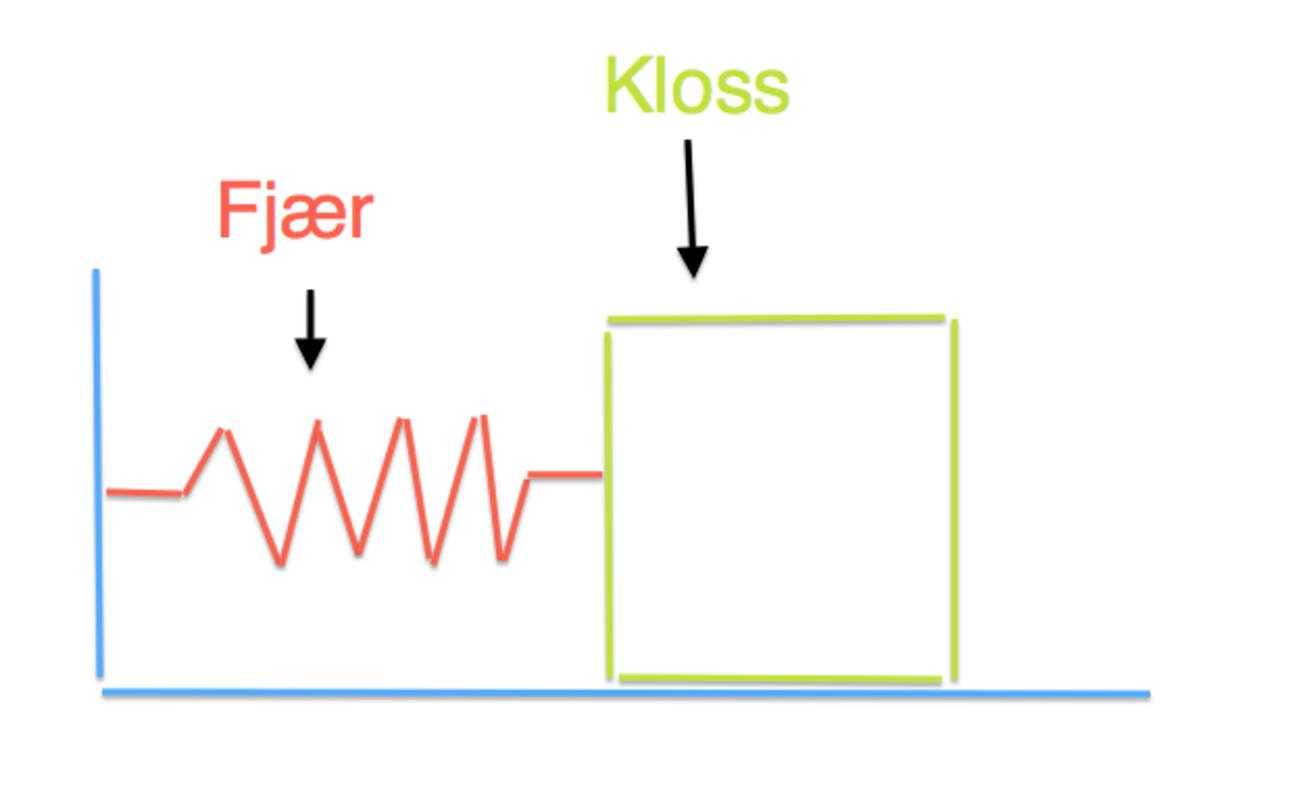
\includegraphics[scale=.35]{Hooke.pdf}
	\label{fig:Num1}
	\end{center}
\end{figure}
\[
F(x)=-kx,
\]
der $x$ er hvor langt fj{\ae}ren er strukket eller komprimert, 
$k$ er en konstant som avhenger av fj{\ae}rens stivhet, 
og $F(x)$ er kraften fra fj{\ae}ren p{\aa} klossen. 
Dersom $x(t)$ er klossens posisjon, er klossens akselerasjon gitt ved $x''(t)$,
og Newtons andre lov blir
\begin{equation*}
-kx=mx'',
\end{equation*}
der $m$ er klossens masse. Dette er en differensiallikning. Vi skriver vanligvis
\[
mx''+kx=0.
\]

Vi kan komplisere det litt til. La oss innf{\o}re luftmotstand. Luftmotstand avhenger kvadratisk av farten:
\begin{equation*}
F(x')=b(x')^{2};
\end{equation*}
der $b$ er en proporsjonalitetskonstant som sier noe om luftmotstanden. 
Den totale kraften blir
\begin{equation*}
F(x,x')=-kx+b(x')^{2},
\end{equation*}
slik at Newtons andre lov gir
\begin{equation*}
mx''-b(x')^{2} +kx=0.
\end{equation*}
Denne likningen har et problematisk ledd, $b(x')^{2}$. Men vi kan gjøre en forenkling. 
Dersom klossen ligger i en tyktflytende væske, blir motstanden proporsjonal med farten istedet for kvadratet av farten, 
og vi får likningen
\begin{equation*}
mx''-cx' +kx=0,
\end{equation*}
som er mye enklere å løse.



N{\aa} skal vi komplisere det enda litt. La klossen henge fra taket.
\begin{figure}[htbp]
  \begin{center}
	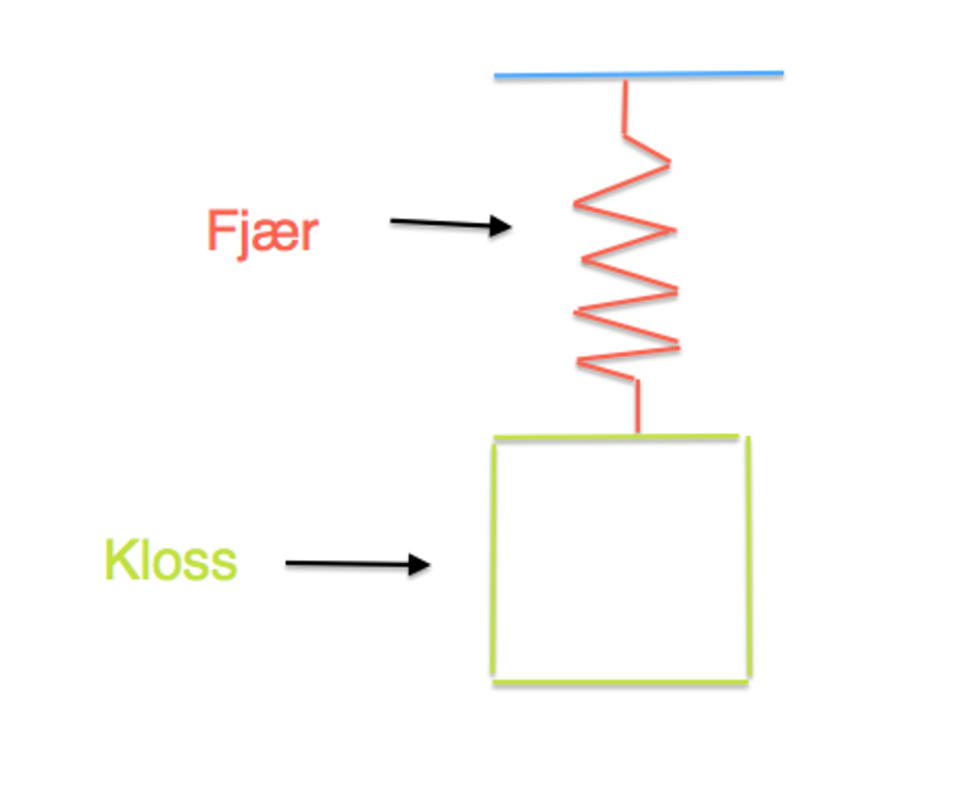
\includegraphics[scale=.4]{Hooke_2.pdf}
	\label{fig:Num1}
	\end{center}
\end{figure}
I tillegg til fj{\ae}rkraften og luftmotstanden, vil n{\aa} ogs{\aa} gravitasjonen p{\aa}virke bevegelsen. Gravitasjonskraften er en konstant kraft $mg$ nedover. Den totale kraften
er
\begin{equation*}
F(x,x')=-kx+bx'-mg,
\end{equation*}
og Newtons andre lov gir differensiallikningen
\begin{equation*}
mx''-bx' +kx=mg.
\end{equation*}





\section*{Omskrivning til system}
En annen ordens differensialikning kan skrives om til et system 
\kapittelslutt
